Gradient backpropagation is the central computational operation of contemporary
deep learning. Its modular structure allows easy extension across network
architectures, and thus automatic computation of gradients given the
computational graph of the forward pass \citep[for a review,
see][]{baydin2018automatic}. But optimization using only the first-order
information of the objective's gradient can be unstable and slow, due to
``vanishing'' or ``exploding'' behaviour of the gradient. Incorporating
curvature, second-order methods can avoid such scaling issues and converge in
fewer iterations. Such methods locally approximate the objective function $\gL$ by
a quadratic
\begin{math}
  \gL(\vtheta) + \grad{\vtheta}\gL(\vtheta)^\top (\vtheta_\star - \vtheta)
  + \nicefrac{1}{2} (\vtheta_\star - \vtheta)^\top \mC(\vtheta) (\vtheta_\star - \vtheta)
\end{math}
around the current location $\vtheta$, using the gradient
$\nabla_{\vtheta}\gL(\vtheta) = \nicefrac{\partial \gL(\vtheta)}{\partial
  \vtheta}$ and a positive semi-definite (PSD) curvature matrix
$\mC(\vtheta)$---the Hessian of $\gL$ or approximations thereof. The quadratic
is minimized by
\begin{align}
  \label{hbp::equ:NewtonUpdate}
  \vtheta_\star = \vtheta
  + \Delta \vtheta
  \quad
  \text{with}
  \quad \Delta \vtheta = -\mC(\vtheta)^{-1} \grad{\vtheta}\gL\,.
\end{align}
Computing the update step requires solving the linear system $\mC(\vtheta)
\Delta \vtheta = -\grad{\vtheta}\gL$. To accomplish this task, providing a
matrix-vector multiplication with the curvature matrix $\mC(\vtheta)$ is
sufficient.

\subsubsection{Approaches to Second-order Optimization}

For some curvature matrices, exact multiplication can be performed at the cost
of one backward pass by automatic differentiation
\citep{pearlmutter1994fast,schraudolph2002fast}. This \emph{matrix-free}
formulation can then be leveraged to solve \Cref{hbp::equ:NewtonUpdate} using
iterative solvers such as conjugate gradients~(CG)~\citep{martens2010deep}.
However, since this linear solver can still require multiple iterations, the
increased per-iteration progress of the resulting optimizer might be compensated
by increased computational cost. Recently, a parallel version of Hessian-free
optimization was proposed in~\citep{zhang2017blockdiagonal}, which only
considers the content of Hessian sub-blocks along the diagonal. Reducing the
Hessian to a block diagonal allows for parallelization, tends to lower the
required number of CG iterations, and seems to improve the optimizer's
performance.

\begin{figure*}[t]
  \centering\resizebox{\linewidth}{!}{
    \tikzexternalenable
    {\footnotesize
      % basic setting of a fully-connected neural network with data flow for
% forward pass

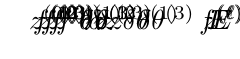
\begin{tikzpicture}
    % first two layers
    \node (in1) 
        [inner sep=0]
        {\tikz \drawMessagesWithArrows{$z^{(0)}$}{ }{ }{\hNodeDistance};};
    \node (layer1)
        [anchor=south west, inner sep=0]
        at (in1.south east)
        {\tikz \drawModuleWithParams{$f^{(1)}$}{16}{$\theta^{(1)}$}{$\delta \theta^{(1)}$}{ };};
    \node (out1)
        [inner sep=0, anchor=south west]
        at (layer1.south east)
        {\tikz \drawMessagesWithArrows{$z^{(1)}$}{$\delta z^{(1)}$}{ }{\hNodeDistance};};
    \node (layer2) 
        [inner sep=0pt, anchor=south west]
        at (out1.south east)
        {\tikz\drawModuleNoParams{$f^{(2)}$}{5};};
    
    % third layer and dots
    \node (in2)
        [inner sep=0, anchor=south west]
        at (layer2.south east)
        {\tikz \drawMessagesWithArrows{$z^{(2)}$}{$\delta z^{(2)}$}{ }{\hNodeDistance};};
    \node (layer3)
        [anchor=south west, inner sep=0]
        at (in2.south east)
        {\tikz \drawModuleWithParams{$f^{(3)}$}{16}{$\theta^{(3)}$}{$\delta \theta^{(3)}$}{ };};
    \node (out3)
        [inner sep=0, anchor=south west]
        at (layer3.south east)
        {\tikz \drawMessagesWithArrows{$z^{(3)}$}{$\delta z^{(3)}$}{ }{\hNodeDistance};};
    \node (layer4)
        [inner sep=0pt, anchor=south west]
        at (out3.south east)
        {\tikz\drawModuleNoParams{$f^{(4)}$}{5};};	

    % last layer after dots
    \node (dots)
        [xshift=2ex, inner sep=0pt, anchor=west]
        at (layer4.east)
        {$\dots$};
    \node (layer5)
        [xshift=12ex, anchor=south west, inner sep=0]
        at (out3.south east)
        {\tikz \drawModuleWithParams{$f^{(\ell)}$}{16}{$\theta^{(\ell)}$}{$\delta \theta^{(\ell)}$}{ };};
    \node (out4)
        [inner sep=0, anchor=south west]
        at (layer5.south east)
        {\tikz \drawMessagesWithArrows{$z^{(\ell)}$}{$\delta z^{(\ell)}$}{ }{\hNodeDistance};};
    
    % loss layer
    \node (lossLayer)
        [inner sep=0pt, anchor=south west]
        at (out4.south east)
        {\tikz\drawModuleNoParams{$E$}{5};};
    \node (loss)
        [inner sep=0, anchor=south west]
        at (lossLayer.south east)
        {\tikz \drawMessagesWithArrows{$E$}{ }{ }{\hNodeDistance};};	
\end{tikzpicture}
    }
    \tikzexternaldisable}
  \caption{\textbf{Standard sequential feedforward network architecture.} \Ie the
    repetition of affine transformations parameterized by $ \vtheta^{(l)} =
    ((\vec \mW^{(l)})^{\top}, \vb^{(l)\top})^{\top}$ followed by element-wise
    activations. Arrows from left to right and vice versa indicate the data flow
    during forward pass and gradient backpropagation, respectively.}
  \label{hbp::fig:setting}
\end{figure*}

There have also been attempts to compute parts of the Hessian in an iterative
fashion \citep{mizutani2008secondorder}. Storing these constituents efficiently
often requires an involved manual analysis of the Hessian's structure,
leveraging its outer-product form in many scenarios
\citep{naumov2017HessianInMatrixForm, bakker2018OuterProductStructure}. Recent
works developed different block-diagonal approximations (BDA) of curvature
matrices that provide fast
multiplication~\citep{martens2015optimizing,grosse2016kronecker,botev2017practical,wei2018bdapch}.

These works have repeatedly shown that, empirically, second-order information
can improve the training of deep learning problems. Perhaps the most important
practical hurdle to the adoption of second-order optimizers is that they tend to
be tedious to integrate in existing ML frameworks because they require manual
implementations. As efficient automated implementations have arguably been more
important for the wide-spread use of deep learning than many conceptual
advances, we aim to develop a framework that makes computation of Hessian
approximations about as easy and automated as gradient backpropagation.

\subsubsection{Contribution}

This chapter introduces a modular formalism for the computation of
block-diagonal approximations of Hessian and curvature matrices, to various
block resolutions, for feedforward neural networks. The framework unifies
previous approaches in a form that, similar to gradient backpropagation, reduces
implementation and analysis to local modules. Following the design pattern of
gradient backprop also has the advantage that this formalism can readily be
integrated into existing ML libraries, and flexibly modified for
different block groupings and approximations.

The framework consists of three principal parts:
\begin{enumerate}
\item A modular formulation for \emph{exact} computation of Hessian block
  diagonals of feedforward neural nets. We achieve a clear presentation by
  leveraging the notation of matrix differential
  calculus~\citep{magnus1999MatrixDifferentialCalculus}.
\item Projections onto the positive semi-definite cone by eliminating sources of
  concavity.
\item Backpropagation strategies to obtain (i) exact curvature matrix-vector
  products (with previously inaccessible BDAs of the Hessian) and (ii) further
  approximated multiplication routines that save computations by evaluating the
  matrix representations of intermediate quantities once, at the cost of
  additional memory consumption.
\end{enumerate}
The first two contributions can be understood as an explicit formulation of
well-known tricks for fast multiplication by curvature matrices using automatic
differentiation~\citep{pearlmutter1994fast,schraudolph2002fast}. However, we
also address a new class of curvature matrices, the positive-curvature Hessian
(PCH) introduced in~\cite{wei2018bdapch}. Our solutions to the latter two points
are generalizations of previous works~\citep{botev2017practical,wei2018bdapch}
to the fully modular case, which become accessible due to the first
contribution. They represent additional modifications to make the scheme
computationally tractable and obtain curvature approximations with desirable
properties for optimization.

%%% Local Variables:
%%% mode: latex
%%% TeX-master: "../thesis"
%%% End:
